\section{Sicherheit}
\label{subsec:sicherheit}

Um die Kommunikation zwischen den Teilnehmern zu schützen, finden sowohl asymmetrische als auch symmetrische Verschlüsselung Anwendung. Die asymmetrische Verschlüsselung wird für die Authentifizierung und die symmetrische Verschlüsselung für die Ende-zu-Ende-Verschlüsselung der Nachrichten verwendet. 

\subsection{Vertrauliche Kommunikation}
\label{subsec:vertrauliche_kommunikation}

Die Kommunikation zwischen den Teilnehmern soll vertraulich sein. Das bedeutet, dass die Nachrichten nur von den Teilnehmern gelesen werden können, die an der Kommunikation beteiligt sind. Um dies gewährleisten zu können, wird eine Ende-zu-Ende-Verschlüsselung verwendet. Ende-zu-Ende-Verschlüsselung ist ein Konzept, das besagt, dass die Nachrichten vom Sender verschlüsselt und erst beim Empfänger wieder entschlüsselt werden \parencite[S. 233-260]{Wong_KryptoPraxis}. Die folgende Abbildung \ref{fig:ende_zu_ende} zeigt den Ablauf einer Ende-zu-Ende-Verschlüsselung.


\begin{figure}[H]
    \centering
    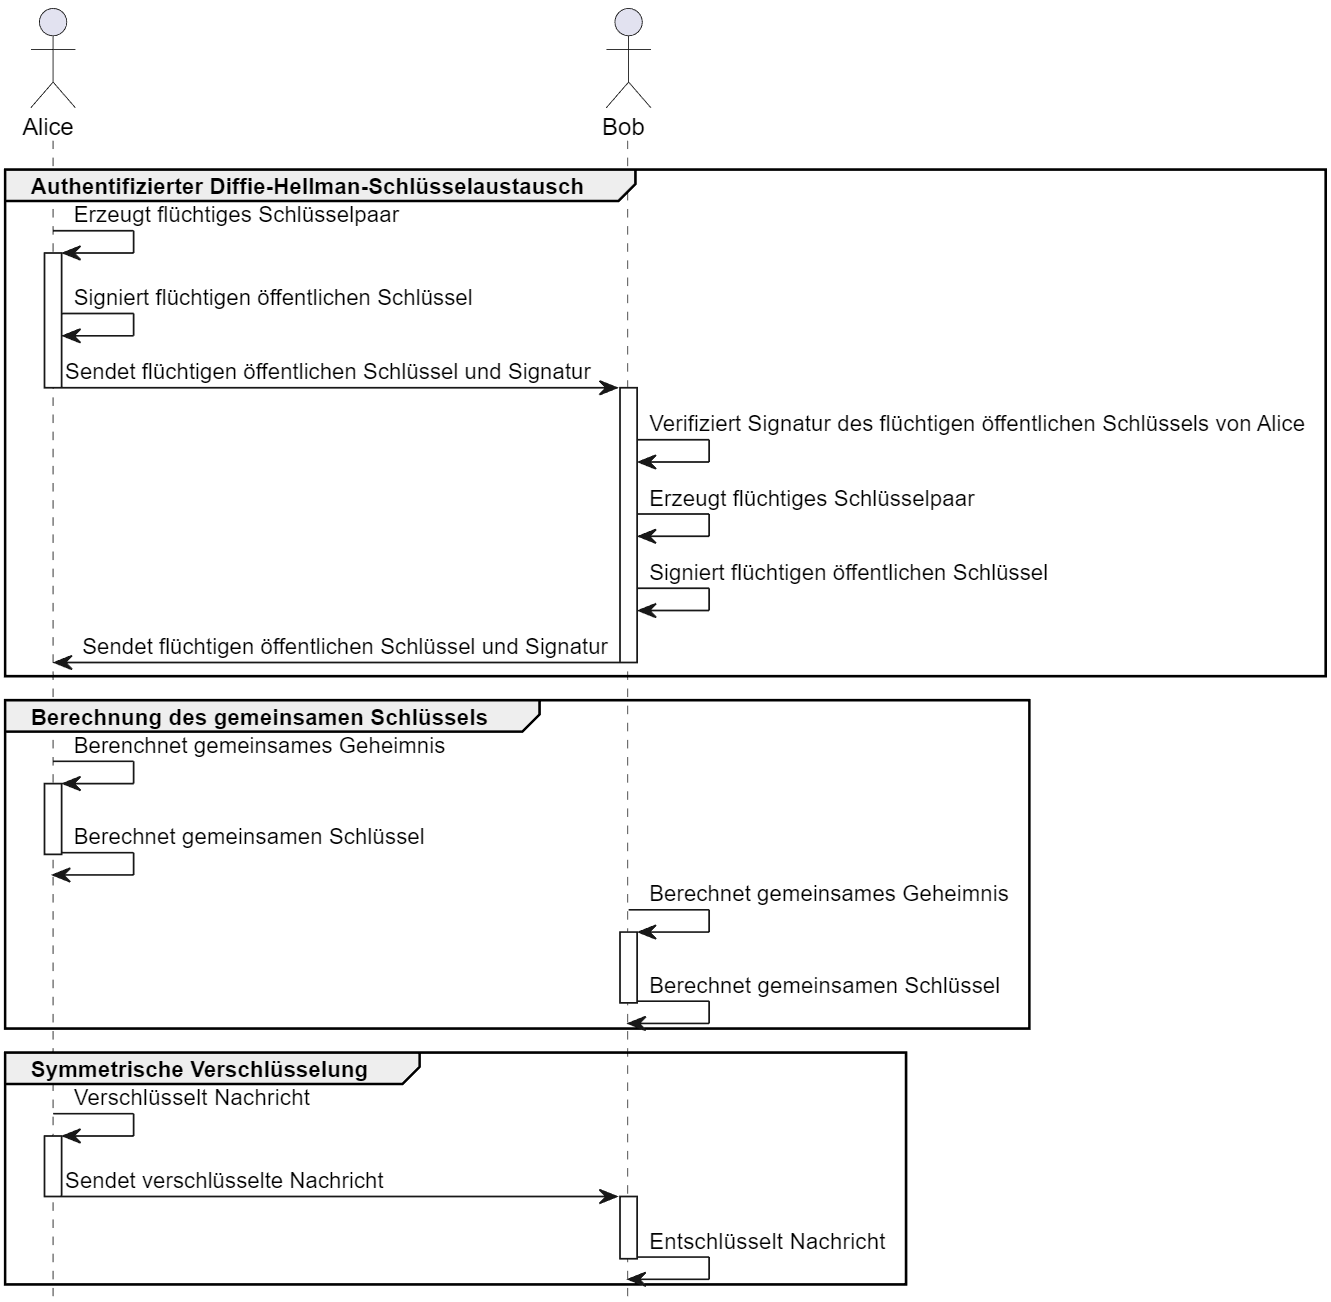
\includegraphics[width=1\linewidth]{images/end2end.png}
    \caption{Ende-zu-Ende-Verschlüsselung}
    \label{fig:ende_zu_ende}
\end{figure}

\noindent In den folgenden Abschnitten werden die Blöcke aus Abbildung \ref{fig:ende_zu_ende} näher erläutert.

\subsubsection{Authentifizierter Diffie-Hellman Schlüsselaustausch}
\label{subsec:ecdh}

Zuerst müssen sich die Teilnehmer auf einen gemeinsamen Schlüssel einigen. Dies nennt man auch \textit{Schlüsselaustausch}. Für die Implementierung eines Schlüsselaustausch kamen zwei Verfahren in Frage. Zum einen der \textit{Diffie-Hellman-(DH-)}Schlüsselaustausch und zum anderen der \textit{Elliptic Curve Diffie-Hellman-(ECDH-)}Schlüsselaustausch. Grundsätzlich baut der Diffie-Hellman-Schlüsselaustausch auf das mathematische Gebiet der \textit{Gruppentheorie} auf. Der DH-Schlüsselaustausch ist ein Schlüsselaustauschverfahren, das auf dem diskreten Logarithmusproblem basiert. Das diskrete Logarithmusproblem ist ein Problem aus der Kryptographie, das besagt, dass es schwierig ist, den Exponenten $x$ zu berechnen, wenn nur die Basis $g$ und das Ergebnis $y$ bekannt sind. Der ECDH-Schlüsselaustausch hingegen basiert auf elliptischen Kurven. David Wong empfiehlt in seinem Buch \textit{Kryptografie in der Praxis} ECDH zu verwenden, da die Schlüssel kleiner sind und noch keine starken Angriffe gegen das Verfahren gefunden wurden \Parencite[S. 101-125]{Wong_KryptoPraxis}.

Aus diesem Grund wurde sich für den ECDH-Schlüsselaustausch entschieden. Hierfür muss eine elliptische Kurve definiert werden. Wong zählt hierfür zwei Kurven auf, die von den meisten Anwendungen verwendet werden: \textit{P-256} und \textit{Curve25519}. Da die Erzeugung der Kurve P-256 unklar ist und damit die Vertrauenswürdigkeit darunter leidet, wurde sich für Curve25519 entschieden \Parencite[S. 121]{Wong_KryptoPraxis}. Den ECDH-Schlüsselaustausch mit Curve25519 nennt man auch X25519 und wird in \cite{rfc_ietf_curve25519} spezifiziert.

Solch ein Schlüsselaustauschverfahren für sich genommen, hat den Nachteil, dass ein aktiver Angreifer die Kommunikation zwischen den Teilnehmern abhören und manipulieren kann. Um dies zu verhindern, wird ein \textit{authentifizierter} Schlüsselaustausch verwendet. Dieser setzt sich zusammen aus dem Schlüsselaustauschverfahren und einer Signatur. Die Signatur wird mit dem privaten statischen Schlüssel des Senders erstellt und kann mit dem öffentlichen statischen Schlüssel des Senders verifiziert werden. Die Wahl eines Signaturverfahrens ist nicht trivial. Wong zählt zwei moderne Verfahren auf: \textit{Elliptic Curve Digital Signature-Algorithmus (ECDSA)} und \textit{Edwards-curve Digital Signature Algorithm (EdDSA)}. Dabei erwähnt er auch Vertrauensbedenken gegenüber ECDSA, weshalb sich für EdDSA entschieden wurde. EdDSA ist ein Signaturverfahren, das auf elliptischen Kurven basiert, weshalb auch hier eine Kurve ausgewählt werden muss. Wong beschreibt, dass in der Praxis meist die Kurve \textit{Edwards25519} verwendet wird. Diese Kombination nennt man auch Ed25519 und wird in \cite{rfc_EdDSA} spezifiziert \Parencite[S. 160-172]{Wong_KryptoPraxis}.

Im Block \textit{Authentifizierter Diffie-Hellman Schlüsselaustausch} aus Abbildung \ref{fig:ende_zu_ende} erzeugt Alice ein neues X25519-Schlüsselpaar und signiert ihren öffentlichen Schlüssel unter Verwendung des privaten statischen Ed25519-Schlüssels. Dieser signierte öffentliche Schlüssel wird an Bob gesendet. Bob erzeugt ebenfalls ein X25519-Schlüsselpaar und signiert seinen öffentlichen Schlüssel mit seinem privaten statischen Ed25519-Schlüssel. Dieser signierte öffentliche Schlüssel wird an Alice gesendet. Alice und Bob können nun das gemeinsame Geheimnis berechnen (siehe \ref{fig:schluesselvereinbarung} \textit{\nameref{fig:schluesselvereinbarung}}).


\subsubsection{Berechnung des gemeinsamen Schlüssels}

Um aus diesem Geheimnis ein möglichst gleichverteiltes Geheimnis zu erzeugen, wird eine \textit{Schlüsselableitungsfunktion} (englisch: \textit{Key Derivation Function}) verwendet. Eine Schlüsselableitungsfunktion ist eine Funktion, die aus einem Eingabeschlüssel (hier das Geheimnis) einen Ausgabeschlüssel erzeugt. Dieser wird dann für die eigentliche Verschlüsselung der Nachricht verwendet. Laut Wong kann dafür eine einfache Hashfunktion (siehe \ref{subsec:vertraulichkeit_basics} \textit{\nameref{subsec:vertraulichkeit_basics}}) verwendet werden, wenn die Ausgabelänge für den Ausgabeschlüssel passend ist \Parencite[S. 194]{Wong_KryptoPraxis}. In diesem Fall wird die \textit{SHA-256} Hashfunktion verwendet, da diese eine Ausgabelänge von $256$ Bit hat \Parencite{rfc6234_SHA2}.

Im Block \textit{Berechnung des gemeinsamen Schlüssels} aus Abbildung \ref{fig:ende_zu_ende} wird das Geheimnis mit der SHA-256 Hashfunktion gehasht und das Ergebnis als symmetrischer Schlüssel verwendet.


\subsubsection{Symmetrische Verschlüsselung}

Der am häufigsten verwendete Verschlüsselungsalgorithmus ist \textit{Advanced Encryption Standard (AES)}. Dieser Algorithmus ist ein symmetrischer Verschlüsselungsalgorithmus (siehe \ref{fig:symmetrische_verschluesselung} \textit{\nameref{fig:symmetrische_verschluesselung}}). Da die Länge des Schlüssels den Grad der Sicherheit bestimmt, wird die maximal mögliche Schlüssellänge von $256$ Bit verwendet \parencite[S. 76]{Wong_KryptoPraxis}. 
Diese Schlüssellänge passt zu der Ausgabelänge der verwendeten Ableitungsfunktion SHA-256.

Im Block \textit{Symmetrische Verschlüsselung} aus Abbildung \ref{fig:ende_zu_ende} wird die Nachricht von Alice mit dem symmetrischen Schlüssel verschlüsselt, signiert und an Bob gesendet. Bob kann die Nachricht mit dem symmetrischen Schlüssel entschlüsseln und die Signatur mit dem öffentlichen statischen Ed25519-Schlüssel von Alice verifizieren.

Dieser Vorgang wird für jede Nachricht wiederholt. Der symmetrische Schlüssel wird für jede Nachricht neu berechnet. Dadurch wird die \textit{Perfect Forward Secrecy} (PFS) gewährleistet. Die PFS ist ein Konzept, welches besagt, dass die Kompromittierung des Schlüssels nicht die Kompromittierung der Kommunikation in der Vergangenheit ermöglichen darf \parencite[S. 921-922]{Krawczyk_PerfectForwardSecrecy}.


\subsubsection{Statische Schlüssel}

Die statischen Schlüssel werden verwendet, um die Teilnehmer zu authentifizieren (Berechnung und Verifikation der Signaturen). Diese Schlüssel werden einmalig bei der Registrierung (siehe \ref{subsec:identifikation_von_teilnehmern} \textit{\nameref{subsec:identifikation_von_teilnehmern}}) eines Teilnehmers erzeugt. Der private Schlüssel wird lokal auf dem Gerät des Teilnehmers gespeichert. Für den öffentlichen Schlüssel muss ein Weg gefunden werden, diesen allen anderen Teilnehmern öffentlich zugänglich und eindeutig zuordenbar zu machen. Hierfür wird die Blockchain verwendet. 


